% LaTeX path to the root directory of the current project, from the directory in which this file resides
% and path to econtexPaths which defines the rest of the paths like \FigDir
\providecommand{\econtexRoot}{}\renewcommand{\econtexRoot}{.}
\providecommand{\econtexPaths}{}\renewcommand{\econtexPaths}{\econtexRoot/Resources/econtexPaths}
% The \commands below are required to allow sharing of the same base code via Github between TeXLive on a local machine and Overleaf (which is a proxy for "a standard distribution of LaTeX").  This is an ugly solution to the requirement that custom LaTeX packages be accessible, and that Overleaf seems to ignore symbolic links (even if they are relative links to valid locations)
\providecommand{\econtex}{\econtexRoot/Resources/texmf-local/tex/latex/econtex}
\providecommand{\econtexSetup}{\econtexRoot/Resources/texmf-local/tex/latex/econtexSetup}
\providecommand{\econtexShortcuts}{\econtexRoot/Resources/texmf-local/tex/latex/econtexShortcuts}
\providecommand{\econtexBibMake}{\econtexRoot/Resources/texmf-local/tex/latex/econtexBibMake}
\providecommand{\econtexBibStyle}{\econtexRoot/Resources/texmf-local/bibtex/bst/econtex}
\providecommand{\econtexBib}{economics}
\providecommand{\notes}{\econtexRoot/Resources/texmf-local/tex/latex/handout}
\providecommand{\handoutSetup}{\econtexRoot/Resources/texmf-local/tex/latex/handoutSetup}
\providecommand{\handoutShortcuts}{\econtexRoot/Resources/texmf-local/tex/latex/handoutShortcuts}
\providecommand{\handoutBibMake}{\econtexRoot/Resources/texmf-local/tex/latex/handoutBibMake}
\providecommand{\handoutBibStyle}{\econtexRoot/Resources/texmf-local/bibtex/bst/handout}

\providecommand{\FigDir}{\econtexRoot/Figures}
\providecommand{\CodeDir}{\econtexRoot/Code}
\providecommand{\DataDir}{\econtexRoot/Data}
\providecommand{\SlideDir}{\econtexRoot/Slides}
\providecommand{\TableDir}{\econtexRoot/Tables}
\providecommand{\ApndxDir}{\econtexRoot/Appendices}

\providecommand{\ResourcesDir}{\econtexRoot/Resources}
\ifnum\pdfshellescape=1
\providecommand{\rootFromOut}{..} % Path back to root directory from output-directory
\providecommand{\LaTeXGenerated}{\econtexRoot/LaTeX} % Put generated files in subdirectory
\providecommand{\EqDir}{\econtexRoot/Equations} % Put generated files in subdirectory
\else
\providecommand{\rootFromOut}{.} % Path back to root directory 
\providecommand{\LaTeXGenerated}{\econtexRoot/} % Put generated files in main directory (because not allowed in subdirectory)
\providecommand{\EqDir}{\econtexRoot/} % Put generated files in main directory
\fi
\providecommand{\econtexPaths}{\econtexRoot/Resources/econtexPaths}
\providecommand{\LaTeXInputs}{\econtexRoot/Resources/LaTeXInputs}

\documentclass[\econtexRoot/BufferStockTheory]{subfiles}
% LaTeX path to the root directory of the current project, from the directory in which this file resides
% and path to econtexPaths which defines the rest of the paths like \FigDir
\providecommand{\econtexRoot}{}\renewcommand{\econtexRoot}{.}
\providecommand{\econtexPaths}{}\renewcommand{\econtexPaths}{\econtexRoot/Resources/econtexPaths}
% The \commands below are required to allow sharing of the same base code via Github between TeXLive on a local machine and Overleaf (which is a proxy for "a standard distribution of LaTeX").  This is an ugly solution to the requirement that custom LaTeX packages be accessible, and that Overleaf seems to ignore symbolic links (even if they are relative links to valid locations)
\providecommand{\econtex}{\econtexRoot/Resources/texmf-local/tex/latex/econtex}
\providecommand{\econtexSetup}{\econtexRoot/Resources/texmf-local/tex/latex/econtexSetup}
\providecommand{\econtexShortcuts}{\econtexRoot/Resources/texmf-local/tex/latex/econtexShortcuts}
\providecommand{\econtexBibMake}{\econtexRoot/Resources/texmf-local/tex/latex/econtexBibMake}
\providecommand{\econtexBibStyle}{\econtexRoot/Resources/texmf-local/bibtex/bst/econtex}
\providecommand{\econtexBib}{economics}
\providecommand{\notes}{\econtexRoot/Resources/texmf-local/tex/latex/handout}
\providecommand{\handoutSetup}{\econtexRoot/Resources/texmf-local/tex/latex/handoutSetup}
\providecommand{\handoutShortcuts}{\econtexRoot/Resources/texmf-local/tex/latex/handoutShortcuts}
\providecommand{\handoutBibMake}{\econtexRoot/Resources/texmf-local/tex/latex/handoutBibMake}
\providecommand{\handoutBibStyle}{\econtexRoot/Resources/texmf-local/bibtex/bst/handout}

\providecommand{\FigDir}{\econtexRoot/Figures}
\providecommand{\CodeDir}{\econtexRoot/Code}
\providecommand{\DataDir}{\econtexRoot/Data}
\providecommand{\SlideDir}{\econtexRoot/Slides}
\providecommand{\TableDir}{\econtexRoot/Tables}
\providecommand{\ApndxDir}{\econtexRoot/Appendices}

\providecommand{\ResourcesDir}{\econtexRoot/Resources}
\ifnum\pdfshellescape=1
\providecommand{\rootFromOut}{..} % Path back to root directory from output-directory
\providecommand{\LaTeXGenerated}{\econtexRoot/LaTeX} % Put generated files in subdirectory
\providecommand{\EqDir}{\econtexRoot/Equations} % Put generated files in subdirectory
\else
\providecommand{\rootFromOut}{.} % Path back to root directory 
\providecommand{\LaTeXGenerated}{\econtexRoot/} % Put generated files in main directory (because not allowed in subdirectory)
\providecommand{\EqDir}{\econtexRoot/} % Put generated files in main directory
\fi
\providecommand{\econtexPaths}{\econtexRoot/Resources/econtexPaths}
\providecommand{\LaTeXInputs}{\econtexRoot/Resources/LaTeXInputs}

\onlyinsubfile{% https://tex.stackexchange.com/questions/463699/proper-reference-numbers-with-subfiles
    \csname @ifpackageloaded\endcsname{xr-hyper}{%
      \externaldocument{\econtexRoot/BufferStockTheory}% xr-hyper in use; optional argument for url of main.pdf for hyperlinks
    }{%
      \externaldocument{main}% xr in use
    }%
    \renewcommand\labelprefix{}%
    % Initialize the counters via the labels belonging to the main document:
    \setcounter{equation}{\numexpr\getrefnumber{\labelprefix eq:AAgg}\relax}% eq:AAgg is the last numbered equation in the main text; start counting up from there
}


\onlyinsubfile{\externaldocument{\LaTeXFiles/BufferStockTheory}} % Get xrefs -- esp to appendix -- from main file; only works properly if main file has already been compiled;
\begin{document}
\let\TableWidth\relax
\newlength\TableWidth
\providecommand{\FigDir}{\econtexRoot/Code/Mathematica/Results/BufferStockTheory/Figures}

\section{Perfect Foresight Liquidity Constrained Solution}\label{sec:ApndxLiqConstr}

Under perfect foresight in the presence of a liquidity constraint requiring $\bRat
\geq 0$, this appendix taxonomizes the varieties of the limiting
consumption function $\grave{\cFunc}(\mRat)$ that arise under various parametric conditions.  Results are summarized in table~\ref{table:LiqConstrScenarios}.

\newsavebox{\LiqConstrScenarios}
\begin{table}[b]
  \centering
  \caption{Taxonomy of Perfect Foresight Liquidity Constrained Model Outcomes}\label{table:LiqConstrScenarios}
  \sbox{\LiqConstrScenarios}{
    \begin{tabular}{|l|rcl|l|}
      \multicolumn{5}{c}{For constrained $\constr{c}$ and unconstrained $\bar{\cFunc}$ consumption functions } \\ \hline
Main Condition     &\multicolumn{3}{c|}{~}         & \\ % & Example \\
~~~~Subcondition   & \multicolumn{3}{c|}{Math}             & \multicolumn{1}{c|}{ Outcome, Comments or Results} % & Example
\\ \hline
\cncl{\PFGIC}      & $\phantom{\Pat/\Rfree}$ & $\phantom{~<~}1        {~<~}$ & $        {\Pat/\PGro}$  & Constraint never binds for $\mRat \geq 1$ %& %$\{\Pat,\PGro\}=\{1,0.98\}$
\\ ~~~~ and \RIC~          & $        {\Pat/\Rfree}$ & $        {~<~}1\phantom{~<~}$ & $\phantom{\Pat/\PGro}$  & ~~~\FHWC~holds ($\Rfree > \PGro$); $\constr{\cFunc}(\mRat) = \bar{\cFunc}(\mRat)$ for $\mRat \geq 1$ % & $\{\Rfree,\Discount, \PGro \} = $
\\ ~~~~ and \cncl{\RIC}   & $\phantom{\Pat/\Rfree}$ & $\phantom{~<~}1        {~<~}$ & $        {\Pat/\Rfree}$ & ~~~~$\constr{\cFunc}(\mRat)$ is degenerate: $\constr{\cFunc}(\mRat)=0$  %&
\\ \PFGIC~            & $        {\Pat/\PGro}$ & $        {~<~}1\phantom{~<~}$ & $\phantom{\Pat/\Rfree}$  & Constraint binds in finite time for any $\mRat$ % &
\\ ~~~~ and \RIC~           & $        {\Pat/\Rfree}$  & $      {~<~}1\phantom{~<~}$ & $\phantom{\Pat/\PGro}$   & ~~~~\FHWC~may or may not hold
\\ ~~~~               &                          &                             &                          & ~~~~~~~$\lim_{m \uparrow \infty}\bar{\cFunc}(\mRat) - \constr{\cFunc}(\mRat) = 0$ % & ~~$\{1.02,1.02^{-1},1.02\}$
\\ ~~~~               &                          &                             &                          & ~~~~~~~$\lim_{m \uparrow \infty}\constr{\MPCFunc}(\mRat) = \MinMPC$ % & ~~$\{1.02,1.02^{-1},1.02\}$
\\ ~~~~ and \cncl{\RIC}   &                          & $\phantom{~<~}1         ~<~ $ & $         \Pat/\Rfree$ & $\cncl{\FHWC}$
\\ ~~~~~~             &                          &                             &                          & ~~~~~$\lim_{\mRat \uparrow \infty} \constr{\MPCFunc}(\mRat) =  0$               % & ~~$\{0.98,1.00, 0.99, 2\} $
\\ \hline
\end{tabular}
} % End \sbox

\settowidth\TableWidth{\usebox{\LiqConstrScenarios}}
\usebox{\LiqConstrScenarios}

\parbox{\TableWidth}{\footnotesize Conditions are applied from left to right; for example, the second row indicates conclusions in the case where \cncl{\PFGIC} and \RIC~both hold, while the third row indicates that when the \PFGIC~and the \RIC~both fail, the consumption function is degenerate; the next row indicates that whenever the \PFGIC~holds, the constraint will bind in finite time.}

\end{table}




\subsection{If \PFGIC~Fails}

A consumer is `growth patient' if the perfect foresight growth
impatience condition fails (\cncl{\PFGIC}, $1 < \Pat/\PGro$).  Under
\cncl{\PFGIC} the constraint does not bind at the lowest feasible value of $\mRat_{t}=1$ because
$1 < (\Rfree\Discount)^{1/\CRRA}/\PGro$ implies that spending
everything today (setting $\cRat_{t}=\mRat_{t}=1$) produces lower
marginal utility than is obtainable by reallocating a marginal unit of
resources to the next period at return $\Rfree$:\footnote{The point at
  which the constraint would bind (if that point could be attained) is
  the $\mRat=\cRat$ for which $\uFunc^{\prime}(\cRat_{\#}) = \Rfree
  \Discount \uFunc^{\prime}(\PGro)$ which is $\cRat_{\#} =
  \PGro/(\Rfree \Discount)^{1/\CRRA}$ and the consumption function
  will be defined by
  $\grave{\cFunc}(\mRat)=\min[\mRat,\cRat_{\#}+(\mRat-\cRat_{\#})\MinMPC
  ]$.}
\begin{align}
  1  & < (\Rfree \Discount)^{1/\CRRA}\PGro^{-1}    \notag
  \\ 1  & < \Rfree \Discount \PGro^{-\CRRA} \notag
  \\  \uFunc^{\prime}(1)  & < \Rfree \Discount \uFunc^{\prime}(\PGro)   \label{eq:EulerPFGICFailsEnd}.
\end{align}

Similar logic shows that under these circumstances the constraint will
never bind at $\mRat=1$ for a constrained consumer with a finite horizon of $n$
periods, so for $\mRat \geq 1$ such a consumer's consumption function will be the same as for the
unconstrained case examined in the main text.

If the \RIC~fails ($1 < \PatR$) while the finite human wealth condition
holds, the limiting value of this consumption function as $n \uparrow
\infty$ is the degenerate function
\begin{align}
  \grave{\cFunc}_{T-n}(\mRat)  & = 0 (\bRat_{t}+\hRat).
\end{align}
(that is, consumption is zero for any level of human or nonhuman wealth).

If the \RIC~fails and the \FHWC~fails, human wealth limits to $\hRat =
\infty$ so the consumption function limits to either
$\grave{\cFunc}_{T-n}(\mRat) = 0$ or
$\grave{\cFunc}_{T-n}(\mRat) = \infty$ depending on the relative
speeds with which the MPC approaches zero and human wealth approaches
$\infty$.\footnote{The knife-edge case is where $\Pat = \PGro$, in
  which case the two quantites counterbalance and the limiting
  function is $\grave{\cFunc}(\mRat)=\min[\mRat,1]$.}

\let\TableWidth\relax
\newlength\TableWidth

Thus, the requirement that the consumption function be nondegenerate
implies that for a consumer satisfying \cncl{\PFGIC} we must impose
the \RIC~(and the \FHWC~can be shown to be a consequence of \cncl{\PFGIC} and \RIC).  In
this case, the consumer's optimal behavior is easy to describe.  We
can calculate the point at which the unconstrained consumer would
choose $\cRat = \mRat$ from equation \eqref{\localorexternallabel{eq:cFuncPFUnc}}:
\begin{align}
  \mRat_{\#}  & = (\mRat_{\#}-1+\hRat)\MinMPC
  \\ \mRat_{\#}(1-\MinMPC)  & = (\hRat - 1)\MinMPC
  \\ \mRat_{\#}  & = (\hRat - 1)\left(\frac{\MinMPC}{1-\MinMPC}\right)
\end{align}
which (under these assumptions) satisfies $0 < \mRat_{\#} < 1$.\footnote{Note that $0 < \mRat_{\#}$ is implied by \RIC~and $ \mRat_{\#}<1$ is implied by \cncl{\PFGIC}.}  For
$\mRat < \mRat_{\#}$ the unconstrained consumer would choose to
consume more than $\mRat$; for such $\mRat$, the constrained consumer
is obliged to choose $\grave{\cFunc}(\mRat) = \mRat$.\footnote{As an
  illustration, consider a consumer for whom $\Pat = 1$, $\Rfree
  =1.01$ and $\PGro = 0.99$.  This consumer will save the amount
  necessary to ensure that growth in market wealth exactly offsets the
  decline in human wealth represented by $\PGro < 1$; total wealth
  (and therefore total consumption) will remain constant, even as
  market wealth and human wealth trend in opposite directions.}  For
any $\mRat > \mRat_{\#}$ the constraint will never bind and the
consumer will choose to spend the same amount as the unconstrained
consumer, $\bar{\cFunc}(\mRat)$.

(\cite{StachurskiToda2019JET} obtain a similar lower bound on consumption and use it to study the tail behavior of the wealth distribution.)


\subsection{If \PFGIC~Holds}

Imposition of the \PFGIC~reverses the inequality in
\eqref{\localorexternallabel{eq:EulerPFGICFailsEnd}}, and thus
reverses the conclusion: A consumer who starts with $\mRat_{t}=1$ will
desire to consume more than 1.  Such a consumer will be constrained,
not only in period $t$, but perpetually thereafter.

Now define $\bRat_{\#}^{n}$ as the $\bRat_{t}$ such that
an unconstrained consumer holding $\bRat_{t}=\bRat_{\#}^{n}$ would behave so as to arrive in period $t+n$ with $\bRat_{t+n}=0$ (with $\bRat_{\#}^{0}$ trivially equal to 0); for example, a consumer with $\bRat_{t-1}=\bRat_{\#}^{1}$ was on the `cusp' of being constrained in period
$t-1$: Had $b_{t-1}$ been infinitesimally smaller, the constraint
would have been binding (because the consumer would have desired, but
been unable, to enter period $t$ with negative, not zero, $b$).  Given
the \PFGIC, the constraint certainly binds in period $t$ (and
thereafter) with resources of
$\mRat_{t}=\mRat_{\#}^{0}=1+\bRat_{\#}^{0}=1$: The consumer cannot
spend more (because constrained), and will not choose to spend less
(because impatient), than $c_{t}=\cRat_{\#}^{0}=1$.

We can construct the entire `prehistory' of this consumer leading up to $t$ as follows.
Maintaining the assumption that the constraint has never bound in the past,
$\cRat$ must have been growing according to $\PatPGro$, so consumption $n$ periods in the past must have been
\begin{align}
  \cRat_{\#}^{n}  & = \PatPGro^{-n} \cRat_{t} = \PatPGro^{-n}. \label{eq:cPreHist}
\end{align}

The PDV of consumption from $t-n$ until $t$ can thus be computed as
\begin{align}
  \mathbb{C}_{t-n}^{t}  & = \cRat_{t-n}(1+\Pat/\Rfree+ ... + (\Pat/\Rfree)^{n}) \notag
  % \\   \mathbb{C}_{t-n}^{t}  & = \cRat_{t-n}(1+\PatPGro/\Rnorm+ ... + (\PatPGro/\Rnorm)^{n}) \notag
  \\  & = \cRat_{\#}^{n}(1+\PatR+ ... + \PatR^{n}) \notag
  \\  & = \PatPGro^{-n}\left(\frac{1-\PatR^{n+1}}{1-\PatR}\right) \label{PDVc}
  \\  & = \left(\frac{\PatPGro^{-n}-\PatR}{1-\PatR}\right) 
\end{align}
and note that the consumer's human wealth between $t-n$ and $t$ (the relevant
time horizon, because from $t$ onward the consumer will be constrained
and unable to access post-$t$ income) is
\begin{align}
  \hRat_{\#}^{n}  & = 1+...+\Rnorm^{-n}
\end{align}
while the intertemporal budget constraint says
\begin{eqnarray*}
  \mathbb{C}_{t-n}^{t}  & = \bRat_{\#}^{n}+\hRat_{\#}^{n}
\end{eqnarray*}
from which we can solve for the $\bRat_{\#}^{n}$ such that
the consumer with $\bRat_{t-n} = \bRat_{\#}^{n}$ would
unconstrainedly plan (in period $t-n$) to arrive in period $t$ with
$\bRat_{t}=0$:
\begin{align}
  \bRat_{\#}^{n} & =  \mathbb{C}_{t-n}^{t} - \overbrace{\left(\frac{1-\Rnorm^{-(n+1)}}{1-\Rnorm^{-1}}\right)}^{\hRat_{\#}^{n}} \label{eq:bPound}.
\end{align}

Defining $\mRat_{\#}^{n}=\bRat_{\#}^{n}+1$, consider the function
$\grave{\cFunc}(\mRat)$ defined by linearly connecting the points
$\{\mRat_{\#}^{n},\cRat_{\#}^{n}\}$ for integer values of $n \geq 0$
(and setting $\grave{\cFunc}(\mRat)=\mRat$ for $\mRat<1$).  This
function will return, for any value of $\mRat$, the optimal value of
$\cRat$ for a liquidity constrained consumer with an infinite horizon.
The function is piecewise linear with `kink points' where the slope
discretely changes; for infinitesimal $\epsilon$ the MPC of a
consumer with assets $\mRat=\mRat_{\#}^{n}-\epsilon$ is discretely
higher than for a consumer with assets $\mRat=\mRat_{\#}^{n}+\epsilon$
because the latter consumer will spread a marginal dollar over more
periods before exhausting it.

In order for a unique consumption function to be defined by this
sequence \eqref{\localorexternallabel{eq:bPound}} for the entire domain of positive real
values of $b$, we need $\bRat_{\#}^{n}$ to become arbitrarily large with
$n$.  That is, we need
\begin{align}
  \lim_{n \rightarrow \infty} \bRat_{\#}^{n} = \infty. \label{eq:bToInfty}
\end{align}

\subsubsection{If \FHWC~Holds}
The \FHWC~requires $\Rnorm^{-1} < 1$, in which case the second term in \eqref{\localorexternallabel{eq:bPound}} limits to a constant as $n \uparrow \infty$, and \eqref{\localorexternallabel{eq:bToInfty}} reduces to a requirement that
\begin{eqnarray*}
  \lim_{n \rightarrow \infty} \left(\frac{\PatPGro^{-n}-(\PatR/\PatPGro)^{n}\PatR}{1-\PatR}\right)  & = \infty
  \\  \lim_{n \rightarrow \infty} \left(\frac{\PatPGro^{-n}-\Rnorm^{-n}\PatR}{1-\PatR}\right)  & = \infty
  \\  \lim_{n \rightarrow \infty} \left(\frac{\PatPGro^{-n}}{1-\PatR}\right)  & = \infty.
\end{eqnarray*}
Given the \PFGIC~$\PatPGro^{-1}>1$, this will hold iff the \RIC~holds, $\PatR < 1$.  But given that the \FHWC~$\Rfree > \PGro$ holds, the \PFGIC~is stronger (harder to satisfy) than the \RIC; thus, the~\FHWC~and the \PFGIC~together imply the \RIC, and so a well-defined
solution exists.  Furthermore, in the limit as $n$ approaches
infinity, the difference between the limiting constrained consumption
function and the unconstrained consumption function becomes
vanishingly small, because the date at which the constraint binds
becomes arbitrarily distant, so the effect of that constraint on current
behavior shrinks to nothing.  That is,
\begin{align}
  \lim_{m \rightarrow \infty}\grave{\cFunc}(m) - \bar{\cFunc}(m) = 0.
\end{align}

% Finally, the main text shows that the \PFGIC~is a stronger condition than the PF-FVR; that is, \PFGIC~$\Rightarrow$ PF-FVR.

\subsubsection{If \FHWC~Fails}
If the \FHWC~fails, matters are a bit more complex.

\begin{comment}
  As noted in the main text, the Finite Value Requirement for such a consumer
  requires $\PatPGro < (\Rfree/\PGro)^{1/\CRRA}$,\footnote{A
    unique well-defined nondegenerate limiting consumption function can
    actually exist even if a nondegenerate value function does not.  But
    the parametric combinations required for this are somewhat peculiar
    (including both $\Rfree < 1$ and $\PGro < 1$); but we restrict our attention
    to the more useful and plausible cases with finite value.} which is stronger (holds
  in strictly fewer circumstances) than the \PFGIC~condition $\PatPGro < 1$.
  Thus, the \PFGIC~is an implication of $\cncl{\FHWC}$.
\end{comment}

Given failure of \FHWC, \eqref{\localorexternallabel{eq:bToInfty}} requires

\begin{align}
  % \lim_{n \rightarrow \infty} \left(\frac{\PatPGro^{-n}-\Rnorm^{-n}\PatR}{1-\PatR}\right) + \left(\frac{1-\Rnorm^{-(n+1)}}{\Rnorm^{-1}-1}\right)  & = \infty \\
  \lim_{n \rightarrow \infty} \left(\frac{\Rnorm^{-n}\PatR-\PatPGro^{-n}}{\PatR-1}\right) + \left(\frac{1-\Rnorm^{-(n+1)}}{\Rnorm^{-1}-1}\right)  & = \infty \notag
  \\   \lim_{n \rightarrow \infty} \left(\frac{\PatR}{\PatR-1}-\frac{\Rnorm^{-1}}{\Rnorm^{-1}-1}\right)\Rnorm^{-n}-\left(\frac{\PatPGro^{-n}}{\PatR-1}\right)  & = \infty \label{eq:FHWCfails} 
  % \\   \lim_{n \rightarrow \infty} \left(\frac{\PatR(\Rnorm^{-1}-1)}{(\Rnorm^{-1}-1)(\PatR-1)}-\frac{\Rnorm^{-1}(\Rnorm^{-1}-1)}{(\Rnorm^{-1}-1)(\PatR-1)}\right)\Rnorm^{-n}-\left(\frac{\PatPGro^{-n}}{\PatR-1}\right)  & = \infty. 
\end{align}
\hypertarget{PFGICHoldsFHWCFailsRICFailsDiscuss}{}

\noindent {\bf If \RIC~Holds}.  When the \RIC~holds, rearranging \eqref{\localorexternallabel{eq:FHWCfails}} gives
\begin{eqnarray*}
  \lim_{n \rightarrow \infty} \left(\frac{\PatPGro^{-n}}{1-\PatR}\right)-\Rnorm^{-n}\left(\frac{\PatR}{1-\PatR}+\frac{\Rnorm^{-1}}{\Rnorm^{-1}-1}\right)  & = \infty
\end{eqnarray*}
and for this to be true we need
\begin{eqnarray*}
  \PatPGro^{-1}  & > \Rnorm^{-1}
  \\ \PGro/\Pat  & > \PGro/\Rfree
  \\ 1  & > \Pat/\Rfree
\end{eqnarray*}
which is merely the \RIC~again.  So the problem has a solution if the \RIC~holds.  Indeed,
we can even calculate the limiting MPC from
\begin{align}
  \lim_{n \rightarrow \infty} \MPC^{n}_{\#}  & = \lim_{n \rightarrow \infty} \left(\frac{\cRat_{\#}^{n}}{\bRat_{\#}^{n}}\right) \label{eq:MPCConstrLim}
\end{align}
which with a bit of algebra\footnote{
  Calculate the limit of
  \begin{align}
    \left(\frac{\PatPGro^{-n}}{\PatPGro^{-n}/(1-\PatR) - (1-\Rnorm^{-1}\Rnorm^{-n})/(1-\Rnorm^{-1})}\right)  & = \left(\frac{1}{1/(1-\PatR) + \Rnorm^{-n}\Rnorm^{-1}/(1-\Rnorm^{-1})}\right)
  \end{align}} can be shown to asymptote to the MPC in the perfect foresight model:\footnote{For an example of this configuration of parameters, see the notebook \texttt{doApndxLiqConstr.nb} in the Mathematica software  archive.}
\begin{align}
  \lim_{m \rightarrow \infty} \grave{\pmb{\MPC}}(\mRat)  & = 1-\PatR.
\end{align}

\noindent {\bf If \RIC~Fails}.  Consider now the \cncl{\RIC} case, $\PatR > 1$.  We can rearrange \eqref{\localorexternallabel{eq:FHWCfails}}as
\begin{eqnarray}
  \lim_{n \rightarrow \infty} \left(\frac{\PatR(\Rnorm^{-1}-1)}{(\Rnorm^{-1}-1)(\PatR-1)}-\frac{\Rnorm^{-1}(\PatR-1)}{(\Rnorm^{-1}-1)(\PatR-1)}\right)\Rnorm^{-n}-\left(\frac{\PatPGro^{-n}}{\PatR-1}\right)  & = \infty.  
\end{eqnarray}
which makes clear that with $\cncl{\FHWC} \Rightarrow \Rnorm^{-1} > 1$ and $\cncl{\RIC} \Rightarrow \PatR > 1$ the numerators and denominators of both terms multiplying $\Rnorm^{-n}$ can be seen transparently to be positive.  So, the terms multiplying
$\Rnorm^{-n}$ in \eqref{\localorexternallabel{eq:FHWCfails}} will be positive if
\begin{eqnarray*}
  \PatR \Rnorm^{-1} - \PatR  & > & \Rnorm^{-1}\PatR-\Rnorm^{-1}
  \\ \Rnorm^{-1}  & > & \PatR
  \\ \PGro  & > & \Pat
\end{eqnarray*}
which is merely the \PFGIC~which we are maintaining.  So the first term's limit is $+\infty$.  The
combined limit will be $+\infty$ if the term involving $\Rnorm^{-n}$
goes to $+\infty$ faster than the term involving $-\PatPGro^{-n}$ goes to
$-\infty$; that is, if
\begin{eqnarray*}
  \Rnorm^{-1}  & > & \PatPGro^{-1}
  \\ \PGro/\Rfree  & > & \PGro/\Pat
  \\ \Pat/\Rfree  & > & 1
\end{eqnarray*}
which merely confirms the starting assumption that the \RIC~fails.

What is happening here is that the $\cRat_{\#}^{n}$ term is increasing backward in time at rate dominated in the limit by $\PGro/\Pat$ while the $\bRat_{\#}$ term is increasing at a rate dominated by $\PGro/\Rfree$ term and
\begin{eqnarray}
  \PGro/\Rfree & > & \PGro/\Pat 
\end{eqnarray}
because $\cncl{\RIC} \Rightarrow \Pat > \Rfree.$

Consequently, while $\lim_{n \uparrow \infty} \bRat_{\#}^{n} = \infty$, the limit of the \textit{ratio} $\cRat_{\#}^{n}/\bRat_{\#}^{n}$ in \eqref{eq:MPCConstrLim} is zero.
Thus, surprisingly, the problem has a well defined solution with
infinite human wealth if the \RIC~fails.  It remains true that \cncl{\RIC}
implies a limiting MPC of zero,
\begin{align}
  \lim_{\mRat \rightarrow \infty} \grave{\pmb{\MPC}}(\mRat)   & = 0,
\end{align}
but that limit is approached gradually, starting from a positive
value, and consequently the consumption function is {\it not} the
degenerate $\grave{\cFunc}(\mRat)=0$.  (Figure~\ref{fig:PFGICHoldsFHWCFailsRICFails} presents an example for $\CRRA=2$, $\Rfree=0.98$, $\Discount = 1.00$, $\PGro = 0.99$; note that the horizontal axis is bank balances $\bRat = \mRat-1$; the part of the consumption function below the depicted points is uninteresting -- $\cRat = \mRat$ -- so not worth plotting).


% \hypertarget{PFGICHoldsFHWCFailsRICFails}{}
\begin{figure}
\centerline{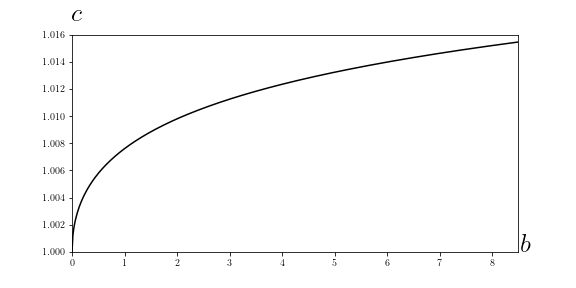
\includegraphics[width=6in]{\FigDir/PFGICHoldsFHWCFailsRICFails}}
\caption{Nondegenerate Consumption Function with $\cncl{\FHWC}$ and \cncl{\RIC}}
\label{fig:PFGICHoldsFHWCFailsRICFails}
\end{figure}

\hypertarget{PFGICHoldsFHWCFailsRICFails}{}
\begin{figure}
\centerline{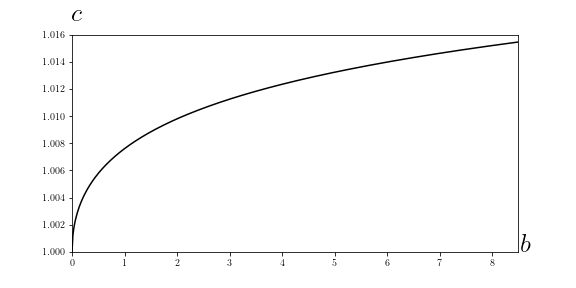
\includegraphics[width=6in]{\FigDir/PFGICHoldsFHWCFailsRICFails}}
\caption{Nondegenerate Consumption Function with $\cncl{\FHWC}$ and \cncl{\RIC}}
\label{fig:PFGICHoldsFHWCFailsRICFails}
\end{figure}



\begin{comment}
  We can rewrite the expression for $\mathbb{C}$ from \eqref{\localorexternallabel{PDVc}} as:
  \begin{eqnarray*}
    \mathbb{C}_{t-n}^{t}  & =  \left(\frac{\PatPGro^{-n}-\PatPGro^{-n}\PatR^{n+1}}{1-\PatR}\right)
    \\  & =  \left(\frac{\PatPGro^{-n}-\PatR\PGro^{n}/\Rfree^{n}}{1-\PatR}\right)
    \\  & =  \left(\frac{(\PGro/\Pat)^{n}-\PatR(\PGro/\Rfree)^{n}}{1-\PatR}\right)
    \\  & =  (\PGro/\Rfree)^{n}\left(\frac{(\Rfree/\Pat)^{n}-\PatR}{1-\PatR}\right)
    \\ \Rnorm^{n}\mathbb{C}_{t-n}^{t}   & =  \left(\frac{(\Rfree/\Pat)^{n}-\PatR}{1-\PatR}\right)
  \end{eqnarray*}
  but \cncl{\RIC} implies that $\Pat > \Rfree$ so
  \begin{eqnarray*}
    \lim_{n \rightarrow \infty} \Rnorm^{n}\mathbb{C}_{t-n}^{t}   & =  \left(\frac{-\PatR}{1-\PatR}\right)
  \end{eqnarray*}
  which means that in the limit
  \begin{align}
    \lim_{n \rightarrow \infty} \Rnorm^{n}\bRat_{\#}^{n}  & =  \left(\frac{-\PatR}{1-\PatR}\right) - \Rnorm^{n}\left(\frac{1-\Rnorm^{-1}\Rnorm^{-n}}{1-\Rnorm^{-1}}\right) %\label{eq:bPoundLim}
    \\  & = \left(\frac{-\PatR}{1-\PatR} + \frac{-\Rnorm^{-1}}{1-\Rnorm^{-1}}\right) - \left(\frac{\Rnorm^{n}}{1-\Rnorm^{-1}}\right)
  \end{align}
  so we can solve for the limiting $n$ as a function of $\bRat$ via
  \begin{align}
    \bRat + \left(\frac{1}{1-\Rnorm^{-1}}\right)  & = \Rnorm^{-\hat{n}}\left(\frac{-\PatR}{1-\PatR} + \frac{-\Rnorm^{-1}}{1-\Rnorm^{-1}}\right)
    \\ \log \left(\bRat + \left(\frac{1}{1-\Rnorm^{-1}}\right)\right)  & = -\hat{n} \log \Rnorm + \log \left(\frac{-\PatR}{1-\PatR} + \frac{-\Rnorm^{-1}}{1-\Rnorm^{-1}}\right)
    \\ \frac{\log \left(\frac{-\PatR}{1-\PatR} + \frac{-\Rnorm^{-1}}{1-\Rnorm^{-1}}\right)-\log \left(\bRat + \left(\frac{1}{1-\Rnorm^{-1}}\right)\right)}{\log \Rnorm }  & = \hat{n}
  \end{align}
  which defines $\hat{\nFunc}(\bRat)$ which yields an approximation to the
  value of $n$ associated with a given $\bRat$.

  We can directly compute
  \begin{align}
    \nabla  & = \bRat - \bRat_{\#}^{\hat{n}}
  \end{align}
  and can obtain a better appxoimation to the correct $n$ from
  \begin{align}
    \hat{\hat{n}} 
    & = \end{align}

  We can obtain a more exact approximation to the correct ${n}$ by defining
  \begin{align}
    \nabla(n) \equiv   \lim_{n \rightarrow \infty}\Rnorm^{n}\mathbb{C}_{t-n}^{t}-\Rnorm^{n}\mathbb{C}_{t-n}^{t}  & =  \left(\frac{\PatR^{-n}}{1-\PatR}\right).
  \end{align}
  from which we can obtain the difference between the approximate and the exact $\mathbb{C}_{t-n}^{t}$ as $\Rnorm^{-n}\nabla(n)$ and


  For this $n$ and
  $\bRat$ we can obtain the corresponding
  $\cRat=\PatPGro^{-\nFunc(\bRat)}$.  Note, however, that this is {\it not}
  the level of $\cRat$ directly associated with $\bRat$ on the true
  consumption function, because we used only a limiting approximation to
  the correct $n$ rather than the correct $n$.

  Our strategy, in this case, is

  The limiting difference can be obtained by realizing that
  \begin{align}
    \nabla(n) \equiv   \lim_{n \rightarrow \infty}\Rnorm^{n}\mathbb{C}_{t-n}^{t}-\Rnorm^{n}\mathbb{C}_{t-n}^{t}  & =  \left(\frac{\PatR^{-n}}{1-\PatR}\right).
  \end{align}
  and so

\end{comment}

We can summarize as follows.  Given that the \PFGIC~holds, the
interesting question is whether the \FHWC~holds.  If so, the
RIC~automatically holds, and the solution limits
into the solution to the unconstrained problem as $\mRat \uparrow
\infty$.  But even if the \FHWC~fails, the problem has a
well-defined and nondegenerate solution, whether or not the \RIC~holds.

Although these results were derived for the perfect foresight case,
we know from work elsewhere in this paper and in other places that the
perfect foresight case is an upper bound for the case with uncertainty.
If the upper bound of the MPC in the perfect foresight case is zero, it
is not possible for the upper bound in the model with uncertainty to be
greater than zero, because for any $\kappa > 0$ the level of consumption
in the model with uncertainty would eventually exceed the level of consumption
in the absence of uncertainty.

\cite{MaTodaMPC} characterize the limits of MPC in a more general framework that allows for non-CRRA utility as well as capital and labor income risks in a Markovian setting, and
find that in that much more general framework the limiting MPC is also zero.

\onlyinsubfile{\pagebreak\bibliography{\LaTeXFiles/BufferStockTheory,economics}}
\end{document}
% Local Variables:
% eval: (setq TeX-command-list  (remove '("Biber" "biber %s" TeX-run-Biber nil  (plain-tex-mode latex-mode doctex-mode ams-tex-mode texinfo-mode)  :help "Run Biber") TeX-command-list))
% eval: (setq TeX-command-list  (remove '("BibTeX" "%(bibtex) %s" TeX-run-BibTeX nil t                                                                              :help "Run BibTeX") TeX-command-list))
% eval: (setq TeX-command-list  (remove '("BibTeX" "%(bibtex) LaTeX/%s" TeX-run-BibTeX nil t                                                                              :help "Run BibTeX") TeX-command-list))
% eval: (setq TeX-command-list  (remove '("BibTeX" "%(bibtex) %s" TeX-run-BibTeX nil (plain-tex-mode latex-mode doctex-mode ams-tex-mode texinfo-mode context-mode) :help "Run BibTeX") TeX-command-list))
% eval: (setq TeX-command-list  (remove '("BibTeX" "%(bibtex) LaTeX/%s" TeX-run-BibTeX nil (plain-tex-mode latex-mode doctex-mode ams-tex-mode texinfo-mode context-mode) :help "Run BibTeX") TeX-command-list))
% eval: (add-to-list 'TeX-command-list	'("BibTeX" "%(bibtex) ../LaTeX/%s" TeX-run-BibTeX nil t :help "Run BibTeX") t)
% TeX-PDF-mode: t
% TeX-file-line-error: t
% TeX-debug-warnings: t
% LaTeX-command-style: (("" "%(PDF)%(latex) %(file-line-error) %(extraopts) -output-directory=../LaTeX %S%(PDFout)"))
% TeX-source-correlate-mode: t
% TeX-source-correlate-start-server: 0
% TeX-parse-self: t
% eval: (cond ((string-equal system-type "darwin") (progn (setq TeX-view-program-list '(("Skim" "/Applications/Skim.app/Contents/SharedSupport/displayline -b %n ../LaTeX/%o %b"))))))
% End:
